% =============================================================================
% DEFINIZIONI VARIABILI
% Comandi che possono cambiare in base alla tipologia di documento o nel corso
% dello sviluppo (es: versioni dei documenti)
% =============================================================================

% Informazini sul documento
% Nome, versione e data del documento
\newcommand{\documentName}{Mancata ridefinizione}
\newcommand{\documentVersion}{Mancata ridefinizione}
\newcommand{\documentDate}{Mancata ridefinizione}

% Responsabili del documento
\newcommand{\documentEditors}{Mancata ridefinizione} % Editori
\newcommand{\documentVerifiers}{Mancata ridefinizione} % Verificatori
\newcommand{\documentApprovers}{Mancata ridefinizione} % Approvatori

% Uso del documento
\newcommand{\documentUsage}{Mancata ridefinizione}

% Destinatari del documento
\newcommand{\documentAddressee}{Mancata ridefinizione}

% Sommario del documento
\newcommand{\documentSummary}{Mancata ridefinizione}

% Dettagli capitolato
\newcommand{\capName}{Mancata ridefinizione} %Nome capitolato
\newcommand{\capCode}{Mancata ridefinizione} %Numero CX
\newcommand{\capLink}{Mancata ridefinizione} %Link pagina prof
\newcommand{\capProposer}{Mancata ridefinizione} % Nome azienda
\newcommand{\capClient}{\Vardanega, \Cardin } % Prof


% Versioni documenti
\newcommand{\docGloVersion}{v0.0.0} % Glossario
\newcommand{\docWowVersion}{v0.0.0} % Way of Working

% =============================================================================
% =============================================================================
% =============================================================================

% ===================================================================
% DEFINIZIONI FISSE
% Non dovrebbe essere necessario andare a ridefinire questi comandi
% =============================================================================

% Informazioni sul gruppo
\newcommand{\groupMail}{\textit{\href{mailto:swemming.pool@gmail.com}{swemming.pool@gmail.com}}}
\newcommand{\groupName}{\textit{SWEmming Pool}}

\newcommand{\groupTeam}{Enrico Bacci Bonivento, Ennio Italiano, Fabio Pantaleo, Elia Pasquali, Sebastiano Sanson, Nicolò Trinca}

\newcommand{\Vardanega}{Prof. Vardanega Tullio}
\newcommand{\vardanega}{Prof. Vardanega}
\newcommand{\Cardin}{Prof. Cardin Riccardo}
\newcommand{\cardin}{Prof. Cardin}

% Ruoli del progetto
\newcommand{\roleProjectManager}{\textit{Responsabile}}
\newcommand{\roleAdministrator}{\textit{Amministratore}}
\newcommand{\roleAnalyst}{\textit{Analista}}
\newcommand{\roleProgrammer}{\textit{Programmatore}}
\newcommand{\roleDesigner}{\textit{Progettista}}
\newcommand{\roleVerifier}{\textit{Verificatore}}

% Nome eventi
\newcommand{\RTB}{\textit{Requirements and Technology Baseline}}
\newcommand{\PB}{\textit{Product Baseline}}
\newcommand{\CA}{\textit{Customer Acceptance}}

% Glossario e relativi
\newcommand{\glo}{\ped{\textbf{\tiny G}}} % Testo glossario

% Documenti, con maiuscola, minuscola e con versione
% Glossario
\newcommand{\docGlo}{\textit{Glossario}}
\newcommand{\Glossario}{\docGlo{} \docGloVersion}

% Way of Working
\newcommand{\docWoW}{\textit{Way of Working}}
\newcommand{\WayOfWorking}{\docWoW{} \docWoWVersion}

% Verbali
\newcommand{\Verbale}{\textit{Verbale}}


\documentclass[11pt,a4paper]{article}
% gestisce i margini ma se attivo fa casino con la prima pagina
\usepackage[a4paper, margin=2.5cm]{geometry}
\usepackage[table]{xcolor}
\usepackage[utf8]{inputenc}
\usepackage[italian]{babel}
\usepackage{alphalph}
\usepackage{longtable}
\usepackage{eurosym}
\usepackage{svg}
\usepackage{graphicx}
\usepackage{import}
\usepackage{listings}
\usepackage{float}
\usepackage{color, colortbl}
\usepackage{markdown}
\usepackage{tabstackengine}
\usepackage{tabularx}
\usepackage{xltabular}
\usepackage{booktabs}
\usepackage{amssymb}
\usepackage{longtable}
\usepackage[T1]{fontenc}
\usepackage{inconsolata}
\usepackage{lastpage}
\usepackage{fancyhdr}
\usepackage{multirow}
\usepackage{caption}

\usepackage{hyperref}
\hypersetup{
    colorlinks=true,
    linkcolor=black,
    urlcolor=blue
}

\setcounter{secnumdepth}{4}
\setcounter{tocdepth}{4}

\definecolor{pari_alt}{HTML}{c9fcfc}
\definecolor{dispari_alt}{HTML}{e3f7f7}
\definecolor{pari}{HTML}{f2f2f2}
\definecolor{dispari}{HTML}{e5e5e5}
\fancypagestyle{stylePage}{
	\thispagestyle{empty}
	\thispagestyle{fancy}
	\pagestyle{fancy}
	%Header	
	\setlength{\topmargin}{-40pt}
	\setlength{\headsep}{60pt}
	\fancyhf{}
	\lhead{SWEmming Pool}
	\setlength{\headheight}{15pt}
	\rhead{
\includegraphics[]{../componenti_comuni/img/logo_swemming.pdf}}
	
	%Footer
	\fancyfoot{}
	\fancyfoot[L]{\documentName}
	\fancyfoot[R]{Pagina \thepage~di~\pageref{LastPage}}
	\futurelet\TMPfootrule\def\footrule{\TMPfootrule}
	\setcounter{page}{0}
	\pagenumbering{arabic}
	\renewcommand{\footrulewidth}{0.3pt}
}

\setcounter{tocdepth}{5} %aggiunge paragrafi e sottoparagrafi ad indice
\setcounter{secnumdepth}{5} %aggiunge numero indicizazzione a paragrafi e sottoparagrafi
\begin{document}
	\renewcommand{\documentName}{Analisi dei requisiti}
	\renewcommand{\documentSummary}{Questo documento presenta i requisiti espliciti ed impliciti ricavati dall'analisi del progetto Trustify e dagli incontri con il proponente.}

	%Prima pagina
	\pagestyle{empty}
	% Informazioni del gruppo
\begin{figure}
    \begin{center}
        
\includegraphics[width=250px]{../componenti_comuni/img/logo_swemming.jpg}
    \end{center}
    \begin{center}
	    \groupMail

\end{center}\end{figure}

% Informazioni sul verbale
\begin{center}
    \textbf{\Large \documentName} \\
    \smallskip
    \textbf{Informazioni sul documento}

    \medskip

    \begin{tabular}{r|l}
        Responsabile & \documentApprovers \\ \smallskip
        Redattori &  \documentEditors \\ \smallskip
        Verificatori & \documentVerifiers \\ \smallskip
        Uso & \documentUsage \\ \smallskip
        Destinatari & \documentAddressee
    \end{tabular}

    \bigskip

    \textbf{Sommario} \\ \documentSummary
\end{center}



	\pagebreak

	%Changelog
	\section*{Diario delle modifiche}

\rowcolors{2}{pari_alt}{dispari_alt}
\renewcommand{\arraystretch}{1.5}
\begin{xltabular}{\textwidth} {
		>{\hsize=0.45\hsize\linewidth=\hsize}X
		>{\hsize=0.7\hsize\linewidth=\hsize}X
		>{\hsize=1.15\hsize\linewidth=\hsize}X
		>{\hsize=0.8\hsize\linewidth=\hsize}X
		>{\hsize=1.85\hsize\linewidth=\hsize}X
	}
	\rowcolorhead
	\textbf{\color{white}Versione} &
	\textbf{\color{white}Data} &
	\textbf{\color{white}Nominativo} &
	\textbf{\color{white}Ruolo} &
	\textbf{\color{white}Descrizione} \\
	\hline
	\endfirsthead

	\hline
	\rowcolorhead
	\textbf{\color{white}Versione} &
	\textbf{\color{white}Data} &
	\textbf{\color{white}Nominativo} &
	\textbf{\color{white}Ruolo} &
	\textbf{\color{white}Descrizione} \\
	\hline
	\endhead

	\endfoot
	\endlastfoot

	2.0.0 &
	2023-05-03 &
	Ennio Italiano&
	Verificatore &
	Aggiunta termini e verifica finale.\\
	\hline

	1.0.0 &
	2023-01-30 &
	Nicolò Trinca&
	Verificatore &
	Verifica glossario.\\
	\hline

	0.1.3 &
	2023-01-23 &
	Sebastiano Sanson\newline
	Enrico Bacci Bonivento&
	Analista \newline Verificatore &
	Aggiunti ulteriori termini norme di progetto.\\
	\hline

	0.1.2 &
	2023-01-13 &
	Elia Pasquali\newline
	Ennio Italiano&
	Analista \newline Verificatore &
	Aggiunti termini \textit{Piano di Progetto}.\\
	\hline

	0.1.1 &
	2022-12-20 &
	Enrico Bacci Bonivento \newline
	Sebastiano Sanson&
	Analista \newline Verificatore &
	Aggiunti termini \textit{Norme di Progetto}. \\
	\hline

	0.1.0 &
	2022-12-16 &
	Nicolò Trinca&
	Verificatore &
	Verifica glossario.\\
	\hline

	0.0.5 &
	2022-12-14 &
	Enrico Bacci Bonivento \newline
	Fabio Pantaleo&
	Analista \newline Verificatore &
	Aggiunti ulteriori termini \textit{Analisi dei Requisiti}. \\
	\hline

	0.0.4 &
	2022-12-13 &
	Elia Paquali\newline
	Sebastiano Sanson&
	Analista \newline Verificatore &
	Aggiunti termini \textit{Piano di Qualifica}. \\
	\hline


	0.0.3 &
	2022-12-05 &
	Fabio Pantaleo \newline
	Elia Paquali&
	Analista \newline Verificatore &
	Aggiunti termini \textit{Analisi dei Requisiti}. \\
	\hline

	0.0.2 &
	2022-11-28 &
	Ennio Italiano \newline
	Sebastiano Sanson&
	Analista \newline Verificatore &
	Aggiunti termini del capitolato. \\
	\hline

	0.0.1 &
	2022-11-22 &
	Ennio Italiano &
	Responsabile &
	Creazione documento. \\
	\hline


\end{xltabular}
\renewcommand{\arraystretch}{1} \pagebreak
	
	%Indici
	\renewcommand{\contentsname}{Contenuti}
	\tableofcontents
	\pagebreak
	\listoffigures
	\listoftables
	\pagebreak

	%Contenuto
	\pagestyle{stylePage}
	\section{Introduzione}
\subsection{Scopo del documento}
Si riporta in questo documento il preventivo per il progetto \textit{Trustify}, calcolato in base alla divisione delle ore di lavoro e relativi costi. \\
I ruoli sono stati divisi tra i vari membri, in modo che ogni partecipante copra tutti i ruoli previsti, calcolando 95 ore produttive per ciascun componente del gruppo.

\input{src/sezioni/qualità_processo}
\input{src/sezioni/qualità_prodotto}
\section{Analisi Dinamica}
\label{sec:analisi_dinamica}

    \subsection{Specifica dei test}
    \begin{itemize}
        \item Test di unità: testano singole componenti del sistema e verranno definiti durante la progettazione di dettaglio;
        \item Test di integrazione: verificano la corretta interazione tra le componenti del sistema e verranno definiti durante la progettazione di dettaglio;
        \item Test di sistema: verificano il corretto funzionamento del sistema per accertare la copertura dei requisiti in preparazione all'accettazione, verranno definiti durante la progettazione di dettaglio;
        \item Test di accettazione: effettuati assieme al proponente durante la fase di collaudo e verranno definiti durante la progettazione di dettaglio.
    \end{itemize}

    \subsection{Test di sistema}

    Nella tabella seguente vengono inseriti i test di sistema per ciascun requisito ed avranno la seguente nomenclatura:\\
    \begin{center}
        \textbf{[TS]+[Codice requisito]}
    \end{center}
    dove TS indica Test di Sistema.
    Si specifica inoltre che i requisiti fanno affidamento alla versione 1.0.2 del documento \textit{Analisi dei requisiti}.


    \renewcommand{\arraystretch}{1.8}
    \begin{xltabular}{\textwidth} {
            >{\hsize=0.6\hsize\linewidth=\hsize}X
            >{\hsize=1.40\hsize\linewidth=\hsize}X
            >{\hsize=1.00\hsize\linewidth=\hsize}X
        }
        \rowcolorhead
        \textbf{\color{white}Codice} &
        \textbf{\color{white}Descrizione} &
        \textbf{\color{white}Implementazione}\\
        \hline
        \endfirsthead

        \hline
        \rowcolorhead
        \textbf{\color{white}Codice} &
        \textbf{\color{white}Descrizione} &
        \textbf{\color{white}Implementazione}\\
        \hline
        \endhead

        \endfoot

        \endlastfoot

        TSR1F1 &
        Si verifica che l'utente non autenticato ha la possibilità di effettuare il login tramite \textit{MetaMask}. &
        Non implementato.
        \\ \hline
        
        TSR1F1.1 &
        Si verifica che in caso di autenticazione fallita venga visualizzato un errore. &
        Non implementato.
        \\ \hline

        TSR1F1.2 &
        Si verifica che in caso di mancata installazione di \textit{MetaMask} venga visualizzato un errore. &
        Non implementato.
        \\ \hline

        TSR1F2&
        [DA RIVEDERE] Si verifica che l'utente autenticato possa eseguire un pagamento tramite \textit{MetaMask} verso un altro indirizzo wallet. &
        Non implementato.
        \\ \hline
        
        TSR1F3&
        Si verifica che l'utente autenticato possa visualizzare un elenco dalla lista di pagamenti effettuati, senza una recensione, dal quale poter scegliere quale recensire.&
        Non implementato.
        \\ \hline

        TSR1F4&
        Si verifica che per acquisti non ancora recensiti, l'utente autenticato ha la possibilità di rilasciare una recensione.&
        Non implementato.
        \\ \hline

        TSR1F4.1&
        Si verifica che per ciascuna transazione esista al massimo una recensione ad essa collegata.&
        Non implementato.
        \\ \hline
        
        TSR1F4.2&
        Si verifica che l'utente possa scegliere la transazione effettuata da associare alla recensione.&
        Non implementato.
        \\ \hline

        TSR1F4.3&
        Si verifica che l'utente abbia inserito un titolo alla recensione.&
        Non implementato.
        \\ \hline

        TSR1F4.4&
        Si verifica che l'utente abbia inserito un voto alla recensione.&
        Non implementato.
        \\ \hline

        TSR1F4.5&
        Si verifica che l'utente abbia inserito un testo alla recensione.&
        Non implementato.
        \\ \hline

        TSR1F4.6&
        Si verifica che venga visualizzato un errore in caso di formato recensione non valido.&
        Non implementato.
        \\ \hline
        
        TSR1F4.6.1&
        Si verifica che la recensione abbia un titolo non superiore ai 50 caratteri.&
        Non implementato.
        \\ \hline

        TSR1F4.6.2&
        Si verifica che la recensione abbia un voto compreso tra 1 e 5.&
        Non implementato.
        \\ \hline

        TSR1F4.6.3&
        Si verifica che la recensione abbia un testo non superiore ai 500 caratteri.&
        Non implementato.
        \\ \hline

        TSR1F5&
        Si verifica che l'utente generico possa ricercare recensioni.&
        Non implementato.
        \\ \hline

        TSR1F5.1&
        Si verifica che l'utente generico possa ricercare recensioni filtrandole per indirizzo wallet.&
        Non implementato.
        \\ \hline
        
        TSR1F5.1.1&
        Si verifica che l'utente generico possa ricercare recensioni filtrandole per indirizzo wallet e per autore.&
        Non implementato.
        \\ \hline
        
        TSR1F5.1.2&
        Si verifica che l'utente generico possa ricercare recensioni filtrandole per indirizzo wallet e per destinatario.&
        Non implementato.
        \\ \hline

        TSR3F5.2&
        Si verifica che l'utente generico possa ricercare recensioni filtrandole per voto.&
        Non implementato.
        \\ \hline
        
        TSR3F5.3&
        Si verifica che l'utente generico possa ricercare recensioni filtrandole per titolo.&
        Non implementato.
        \\ \hline

        TSR3F5.4&
        Si verifica che l'utente generico possa ricercare recensioni filtrandole per data.&
        Non implementato.
        \\ \hline

        TSR1F6&
        Si verifica che l'utente autenticato possa ricercare recensioni rilasciate. &
        Non implementato.
        \\ \hline

        TSR1F7&
        Si verifica che l'utente autenticato possa ricercare recensioni ricevute. &
        Non implementato.
        \\ \hline
        
        TSR1F8&
        Si verifica che venga visualizzato un errore quando la ricerca non va a buon fine. &
        Non implementato.
        \\ \hline

        TSR1F8.1&
        Si verifica che venga visualizzato un errore quando la ricerca per indirizzo wallet non va a buon fine. &
        Non implementato.
        \\ \hline
        
        TSR3F8.2&
        Si verifica che venga visualizzato un errore quando la ricerca per voto non va a buon fine. &
        Non implementato.
        \\ \hline
        
        TSR3F8.3&
        Si verifica che venga visualizzato un errore quando la ricerca per titolo non va a buon fine. &
        Non implementato.
        \\ \hline

        TSR3F8.4&
        Si verifica che venga visualizzato un errore quando la ricerca per data non va a buon fine. &
        Non implementato.
        \\ \hline

        TSR1F9 &
        Si verifica che l'utente generico abbia la possibilità di visualizzare una lista di recensioni.  &
        Non implementato.
        \\ \hline

        TSR1F10 &
        Si verifica che l'utente generico abbia la possibilità di visualizzare una singola recensione. &
        Non implementato.
        \\ \hline

        TSR1F10.1 &
        Si verifica che l'utente generico abbia la possibilità di visualizzare l'autore di una singola recensione.  &
        Non implementato.
        \\ \hline

        TSR1F10.2 &
        Si verifica che l'utente generico abbia la possibilità di visualizzare il destinatario di una singola recensione.  &
        Non implementato.
        \\ \hline

        TSR1F10.3 &
        Si verifica che l'utente generico abbia la possibilità di visualizzare il titolo di una singola recensione.  &
        Non implementato.
        \\ \hline

        TSR1F10.4 &
        Si verifica che l'utente generico abbia la possibilità di visualizzare la data di una singola recensione.  &
        Non implementato.
        \\ \hline
        
        TSR1F10.5 &
        Si verifica che l'utente generico abbia la possibilità di visualizzare il voto di una singola recensione.  &
        Non implementato.
        \\ \hline

        TSR1F10.6 &
        Si verifica che l'utente generico abbia la possibilità di visualizzare il testo di una singola recensione.  &
        Non implementato.
        \\ \hline

        TSR1F11 &
        Si verifica che l'utente autenticato abbia la possibilità di visualizzare le recensioni rilasciate.  &
        Non implementato.
        \\ \hline

        TSR1F12 &
        Si verifica che l'utente autenticato abbia la possibilità di visualizzare le recensioni ricevute.  &
        Non implementato.
        \\ \hline

        TSR1F13 &
        Si verifica che venga notificato un errore nella visualizzazione delle recensioni.  &
        Non implementato.
        \\ \hline

        TSR1F14 &
        Si verifica che il server API REST fornisca all'utente la possibilità di visualizzare le recensioni a lui riferite. &
        Non implementato.
        \\ \hline

        TSR1F15 &
        Si verifica che il server API REST notifichi un errore all'utente in caso di assenza di recensioni a lui collegate. &
        Non implementato.
        \\ \hline


        TSR1F16 &
        Si verifica che l'utente abbia la possibilità visualizzare la lista di tutti i pagamenti
        effettuati. &
        Non implementato.
        \\ \hline

        TSR1F17 &
        Si verifica che l'utente autenticato possa visualizzare una singola transazione. &
        Non implementato.
        \\ \hline

        TSR1F17.1 &
        Si verifica che l'utente autenticato possa visualizzare l'ID di una singola transazione. &
        Non implementato.
        \\ \hline


        TSR1F17.2 &
        Si verifica che l'utente autenticato possa visualizzare la data di una singola transazione. &
        Non implementato.
        \\ \hline

        TSR1F17.3 &
        Si verifica che l'utente autenticato possa visualizzare l'importo di una singola transazione. &
        Non implementato.
        \\ \hline

        TSR1F17.4 &
        Si verifica che l'utente autenticato possa visualizzare l'utente pagante di una transazione. &
        Non implementato.
        \\ \hline

        TSR1F17.5 &
        Si verifica che l'utente autenticato possa visualizzare il destinatario di una transazione. &
        Non implementato.
        \\ \hline

        TSR1F18 &
        Si verifica che l'utente autenticato sia avvisato in caso di errore di visualizzazione dei pagamenti. &
        Non implementato.
        \\ \hline

        TSR1F19 &
        Si verifica che la web app fornisca all'utente generico la possibilità di visualizzare una lista di recensioni ordinate. &
        Non implementato. 
        \\ \hline

        TSR1F19.1 &
        Si verifica che la web app fornisca all'utente generico la possibilità di visualizzare una lista di recensioni ordinate dal meno recente. &
        Non implementato. 
        \\ \hline

        TSR1F19.2 &
        Si verifica che la web app fornisca all'utente generico la possibilità di visualizzare una lista di recensioni ordinate dal più recente. &
        Non implementato. 
        \\ \hline

        TSR1F20 &
        Si verifica che la web app fornisca all'utente generico la possibilità di visualizzare una lista di pagamenti ordinati in base alla data del pagamento. &
        Non implementato. 
        \\ \hline

        TSR1F20.1 &
        Si verifica che l'utente abbia la possibilità di visualizzare la lista di tutti i pagamenti
        effettuati, ordinandoli dal meno recente. &
        Non implementato.
        \\ \hline

        TSR1F20.2 &
        Si verifica che l'utente abbia la possibilità di visualizzare la lista di tutti i pagamenti
        effettuati, ordinandoli dal più recente. &
        Non implementato.
        \\ \hline

        TSR1F21 &
        Si verifica che la web app fornisca all'utente generico la possibilità di visualizzare una lista di pagamenti ordinati in base all'importo del pagamento. &
        Non implementato. 
        \\ \hline

        TSR1F21.1 &
        Si verifica che l'utente abbia la possibilità visualizzare la lista di tutti i pagamenti
        effettuati, ordinandoli per importo più economico. &
        Non implementato.
        \\ \hline
        
        TSR1F21.2 &
        Si verifica che l'utente abbia la possibilità visualizzare la lista di tutti i pagamenti
        effettuati, ordinandoli per importo meno economico. &
        Non implementato.
        \\ \hline


        \rowcolor{white}
        \caption{Test di sistema}
    \end{xltabular}

    \subsection{Tracciamento dei requisiti}

    \renewcommand{\arraystretch}{1.8}
    \begin{xltabular}{\textwidth} {
            >{\hsize=1\hsize\linewidth=\hsize}X
            >{\hsize=1\hsize\linewidth=\hsize}X
        }
        \rowcolorhead
        \textbf{\color{white}Codice test} &
        \textbf{\color{white}Codice requisito}\\
        \hline
        \endfirsthead

        \hline
        \rowcolorhead
        \textbf{\color{white}Codice test} &
        \textbf{\color{white}Codice requisito} \\
        \hline
        \endhead

        \endfoot

        \endlastfoot

        TSR1F1 &
        R1F1
        \\ \hline
        
        TSR1F1.1 &
        R1F1.1
        \\ \hline

        TSR1F1.2 &
        R1F1.2
        \\ \hline

        TSR1F2&
        R1F2
        \\ \hline
        
        TSR1F3&
        R1F3
        \\ \hline

        TSR1F4&
        R1F4
        \\ \hline

        TSR1F4.1&
        R1F4.1
        \\ \hline
        
        TSR1F4.2&
        R1F4.2
        \\ \hline

        TSR1F4.3&
        R1F4.3
        \\ \hline
        
        TSR1F4.4&
        R1F4.4
        \\ \hline

        TSR1F4.5&
        R1F4.5
        \\ \hline

        TSR1F4.6&
        R1F4.6
        \\ \hline
        
        TSR1F4.6.1&
        R1F4.6.1
        \\ \hline

        TSR1F4.6.2&
        R1F4.6.2
        \\ \hline

        TSR1F4.6.3&
        R1F4.6.3
        \\ \hline

        TSR1F5&
        R1F
        \\ \hline

        TSR1F5.1&
        R1F5.1
        \\ \hline
        
        TSR1F5.1.1&
        R1F5.1.1
        \\ \hline
        
        TSR1F5.1.2&
        R1F5.1.2
        \\ \hline

        TSR3F5.2&
        R3F5.2
        \\ \hline
        
        TSR3F5.3&
        R3F5.3
        \\ \hline

        TSR3F5.4&
        R3F5.4
        \\ \hline

        TSR1F6&
        R1F6
        \\ \hline

        TSR1F7&
        R1F7
        \\ \hline
        
        TSR1F8&
        R1F8
        \\ \hline

        TSR1F8.1&
        R1F8.1
        \\ \hline
        
        TSR3F8.2&
        R3F8.2
        \\ \hline
        
        TSR3F8.3&
        R3F8.3
        \\ \hline

        TSR3F8.4&
        R3F8.4
        \\ \hline

        TSR1F9&
        R1F9
        \\ \hline

        TSR1F10&
        R1F10
        \\ \hline
        
        TSR1F10.1 &
        R1F10.1
        \\ \hline
        
        TSR1F10.2 &
        R1F10.2
        \\ \hline

        TSR1F10.3 &
        R1F10.3
        \\ \hline

        TSR1F10.4 &
        R1F10.4
        \\ \hline

        TSR1F10.5 &
        R1F10.5
        \\ \hline

        TSR1F10.6 &
        R1F10.6
        \\ \hline

        TSR1F11 &
        R1F11
        \\ \hline

        TSR1F12 &
        R1F12
        \\ \hline

        TSR1F13 &
        R1F13
        \\ \hline

        TSR1F14 &
        R1F14
        \\ \hline

        TSR1F15 &
        R1F15
        \\ \hline


        TSR1F16 &
        R1F16
        \\ \hline

        TSR1F17 &
        R1F17
        \\ \hline

        TSR1F17.1 &
        R1F17.1
        \\ \hline


        TSR1F17.2 &
        R1F17.2
        \\ \hline

        TSR1F17.3 &
        R1F17.3
        \\ \hline

        TSR1F17.4 &
        R1F17.4
        \\ \hline

        TSR1F17.5 &
        R1F17.5
        \\ \hline

        TSR1F18 &
        R1F18
        \\ \hline

        TSR1F19 &
        R1F19
        \\ \hline

        TSR1F19.1 &
        R1F19.1
        \\ \hline

        TSR1F19.2 &
        R1F19.2
        \\ \hline

        TSR1F20 &
        R1F20
        \\ \hline

        TSR1F20.1 &
        R1F20.1
        \\ \hline

        TSR1F20.2 &
        R1F21.2 
        \\ \hline

        TSR1F21 &
        R1F21
        \\ \hline

        TSR1F21.1 &
        R1F21.1
        \\ \hline

        TSR1F21.2 &
        R1F21.2
        \\ \hline

        \rowcolor{white}
        \caption{Test di sistema con tracciamento dei requisiti}
    \end{xltabular}

    \pagebreak
\section{Resoconto attività di verifica}
\subsection{Periodo di analisi}
In questo paragrafo vengono analizzate le metriche \textit{MPC01, MPC02, MPC03, MPC04, MPC05, MPD01}, i restanti verranno analizzati nela successiva fase di progettazione e codifica.
\subsubsection{MPC01}
Rappresenta il valore delle attività realizzate alla data corrente.
Sull'asse delle ascisse troviamo l'unità di tempo in settimane, mentre in quello delle ordinate il valore in euro.
\begin{figure}[H]
\centering
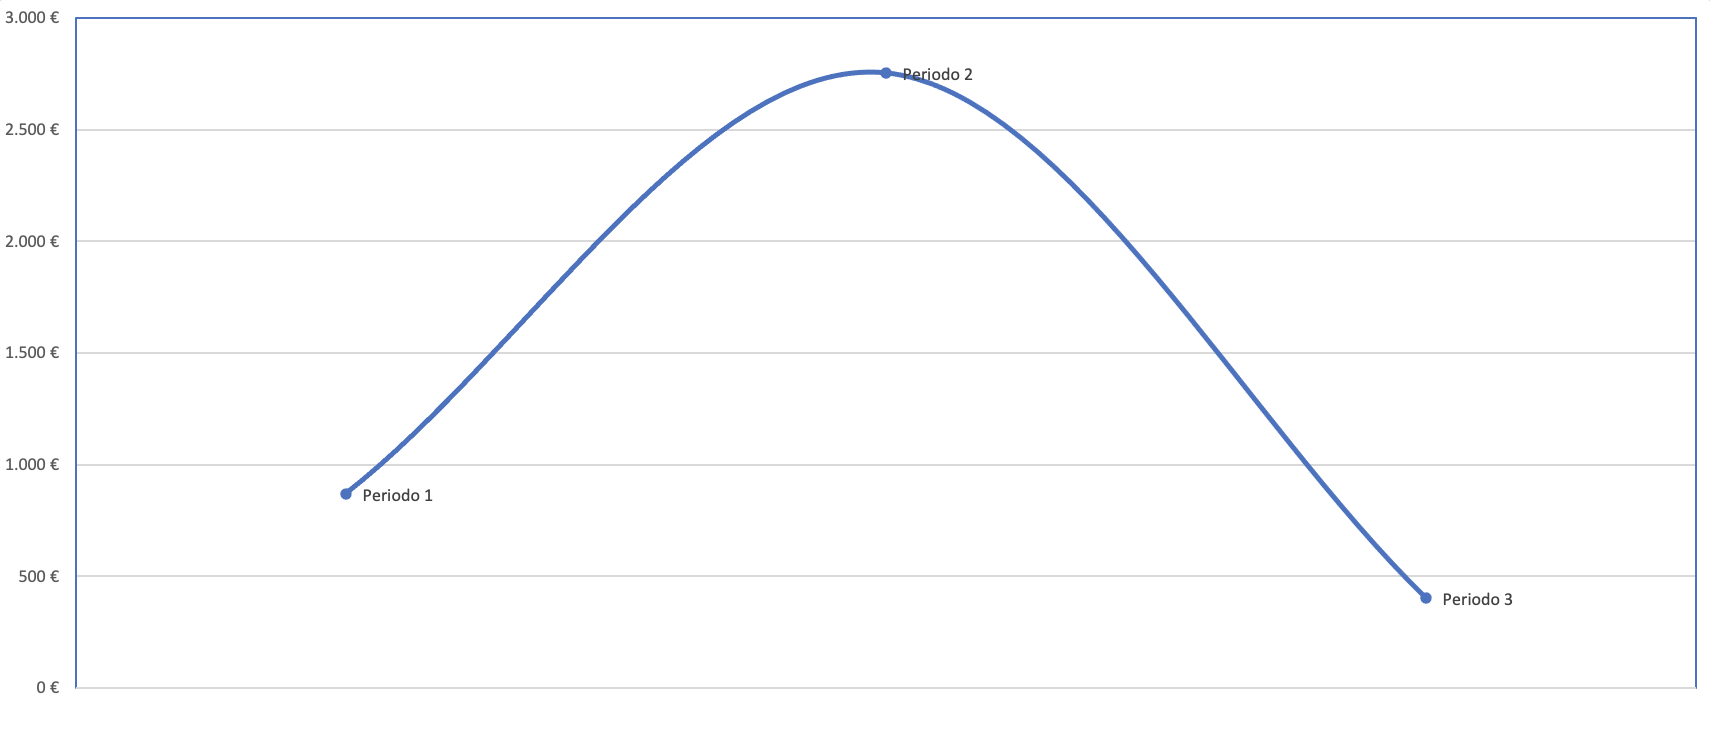
\includegraphics[width=1\textwidth]{src/img/grafico_EV.png}
\caption{Grafico EV}
\end{figure}

\subsubsection{MPC02}
Rappresenta il costo effettivamente sostenuto alla data corrente.
Sull'asse delle ascisse troviamo l'unità di tempo in settimane, mentre in quello delle ordinate il valore in euro.
\begin{figure}[H]
\centering
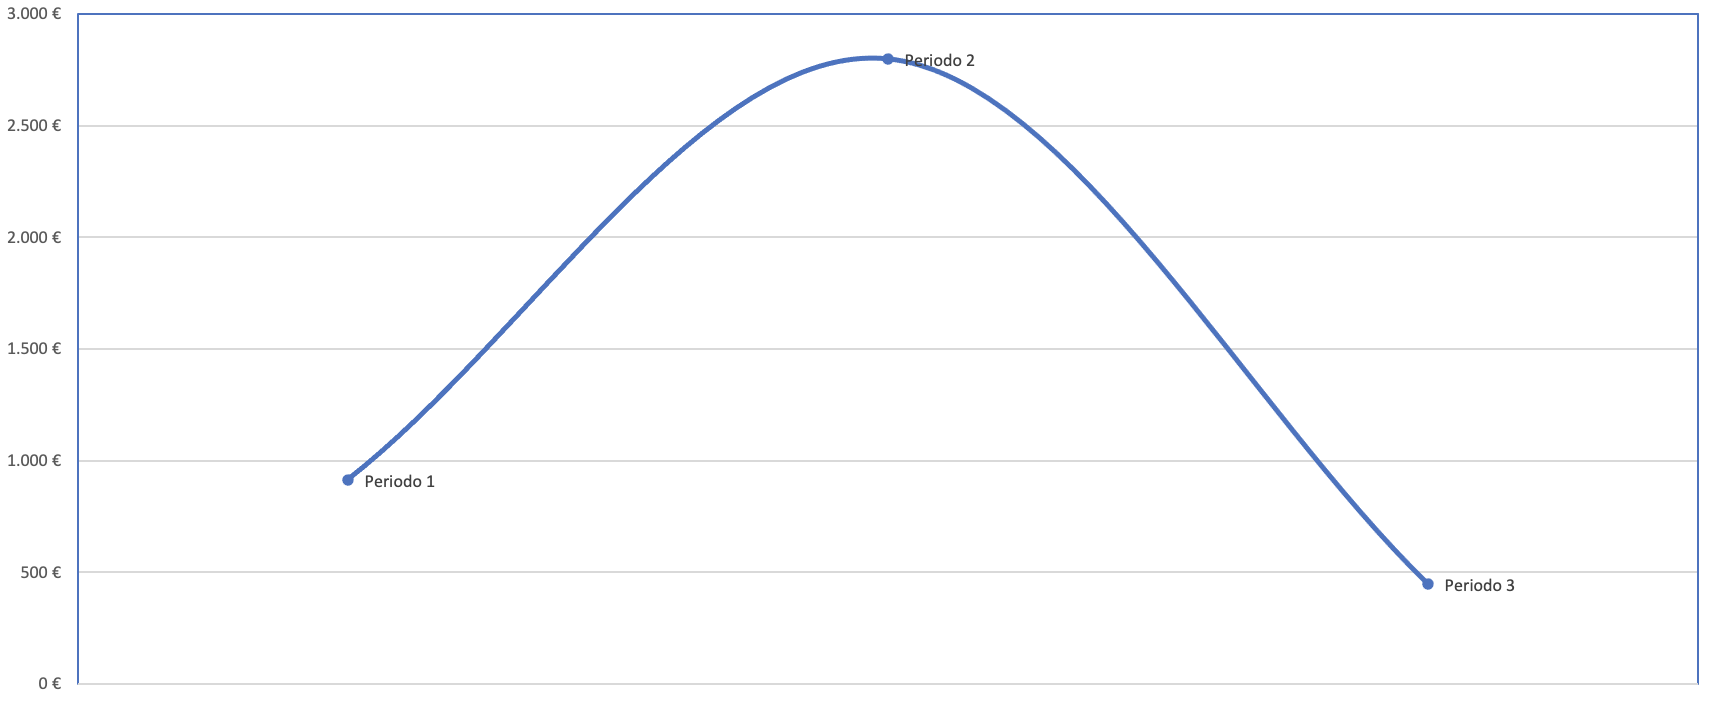
\includegraphics[width=1\textwidth]{src/img/grafico_AC.png}
\caption{Grafico AC}
\end{figure}

\subsubsection{MPC03}
Rappresenta il costo pianificato per realizzare le attività di progetto alla data corrente.
Sull'asse delle ascisse troviamo l'unità di tempo in settimane, mentre in quello delle ordinate il valore in euro.
\begin{figure}[H]
\centering
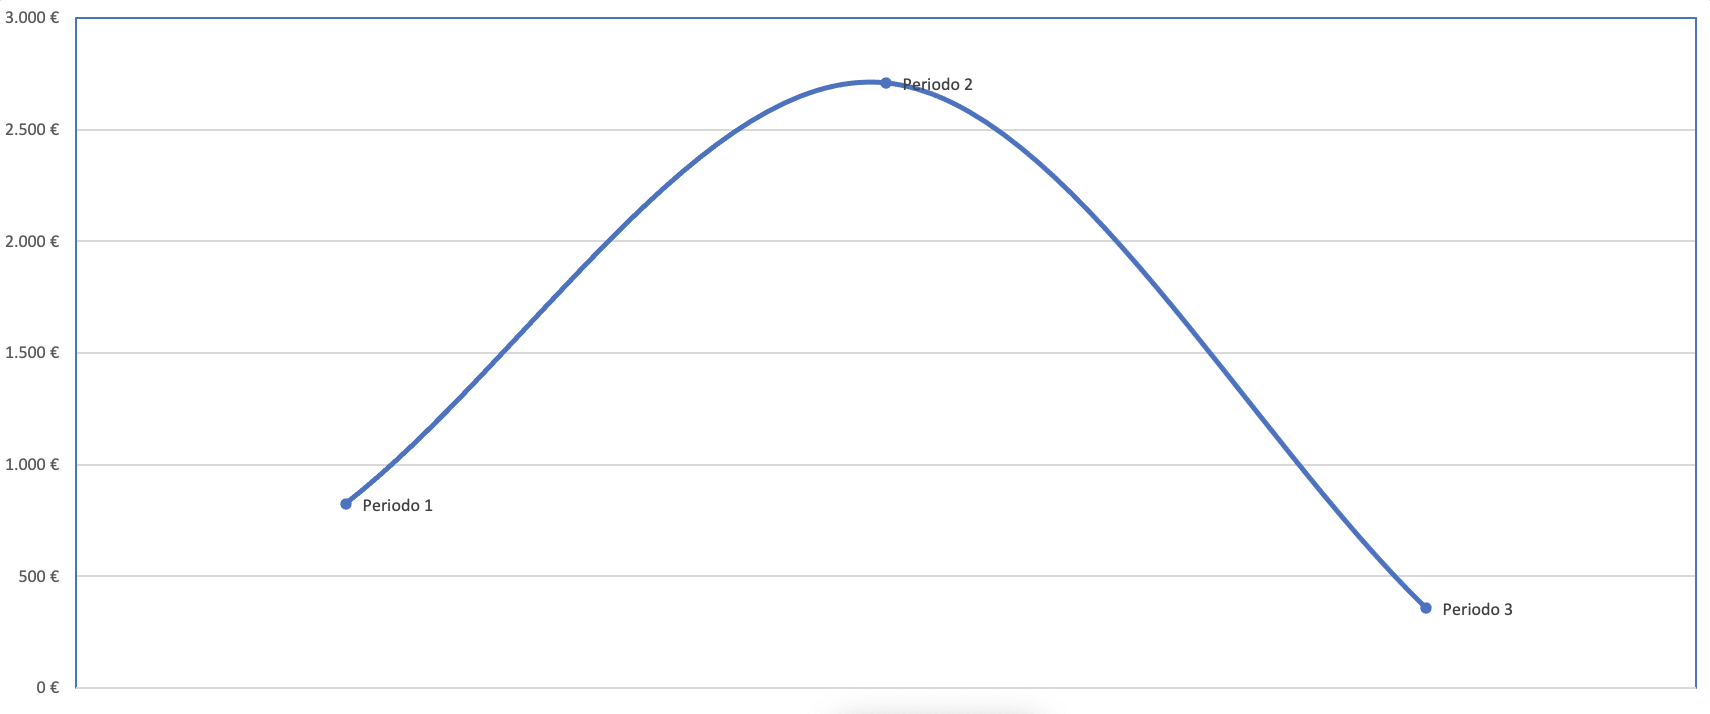
\includegraphics[width=1\textwidth]{src/img/grafico_PV.png}
\caption{Grafico PV}
\end{figure}

\subsubsection{MPC04}
Indica se il valore del costo realmente maturato è maggiore, uguale o minore rispetto al costo effettivo.
Sull'asse delle ascisse troviamo l'unità di tempo in settimane, mentre in quello delle ordinate la variazione in percentuale.
\begin{figure}[H]
\centering
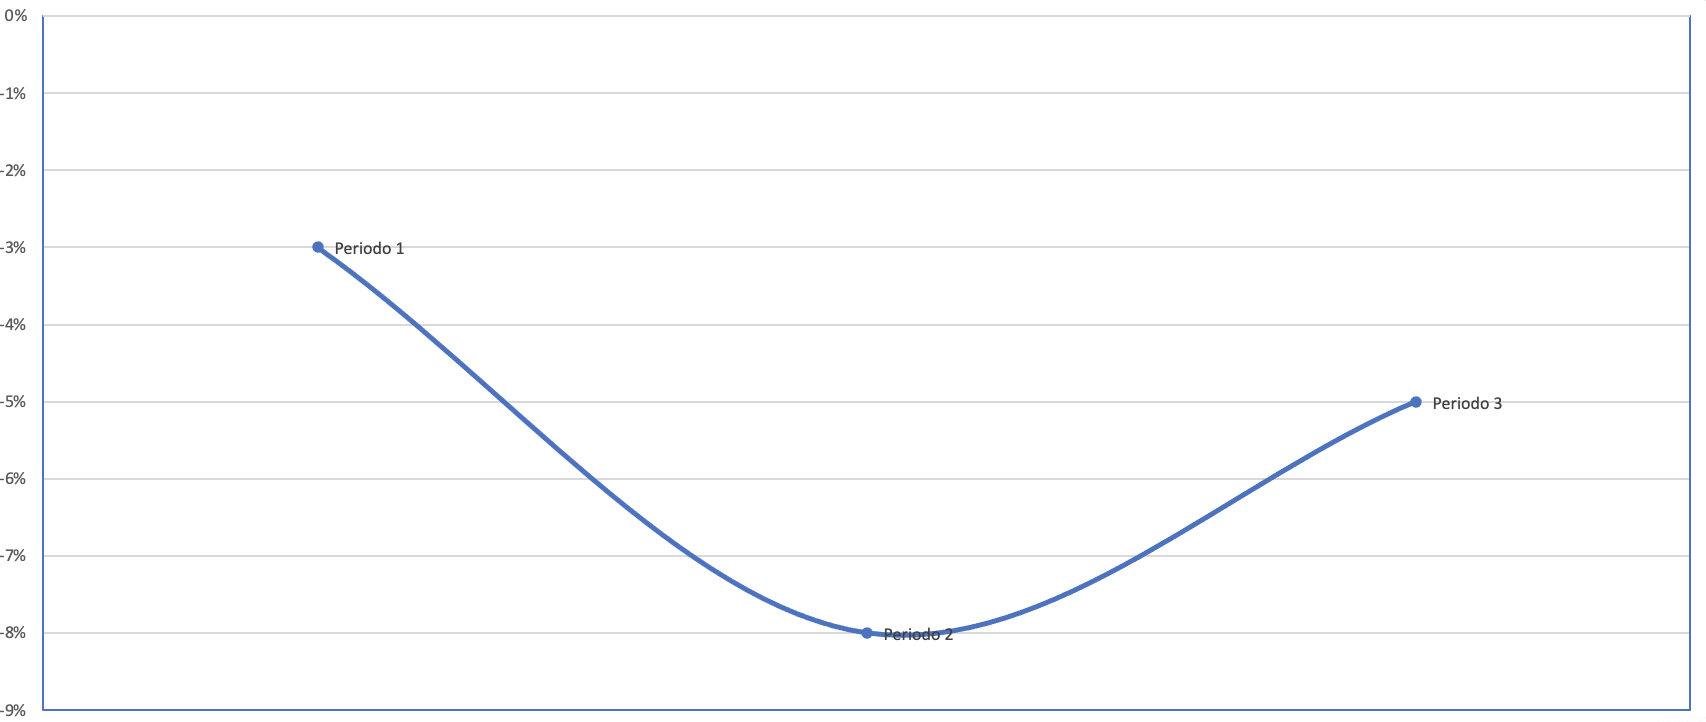
\includegraphics[width=1\textwidth]{src/img/grafico_CV.png}
\caption{Grafico CV}
\end{figure}

\subsubsection{MPC05}
Indica se si è in linea, in anticipo o in ritardo rispetto alla schedulazione delle attività di progetto pianificate nella baseline.
Sull'asse delle ascisse troviamo l'unità di tempo in settimane, mentre in quello delle ordinate la variazione in percentuale.
\begin{figure}[H]
\centering
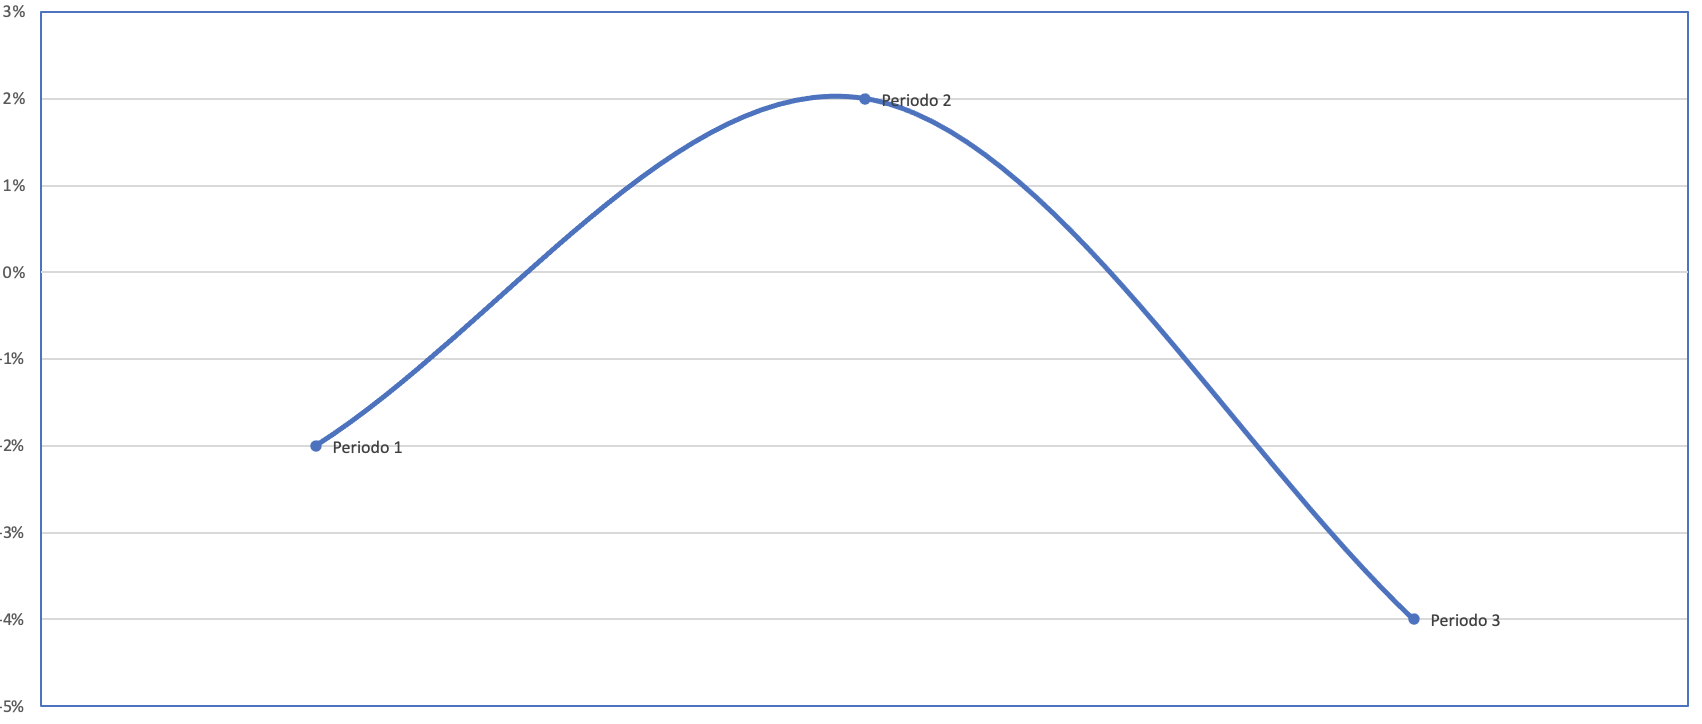
\includegraphics[width=1\textwidth]{src/img/grafico_SV.png}
\caption{Grafico SV}
\end{figure}

\subsubsection{MPD01}
L'Indice Gulpease è un indice di leggibilità di un testo tarato sulla lingua italiana. Rispetto ad altri ha il vantaggio di utilizzare la lunghezza delle parole in lettere anziché in sillabe, semplificandone il calcolo automatico.
I risultati sono compresi tra 0 e 100, dove il valore "100" indica la leggibilità più alta e "0" la leggibilità più bassa. In generale risulta che testi con un indice
\begin{itemize}
    \item inferiore a 80 sono difficili da leggere per chi ha la licenza elementare;
    \item inferiore a 60 sono difficili da leggere per chi ha la licenza media;
    \item inferiore a 40 sono difficili da leggere per chi ha un diploma superiore.
\end{itemize}

Di seguito vengono mostrati i risultati dell’indice di Gulpease per ogni documento redatto, escludendone la prima pagina, registro delle modifiche, l'indice e gli elenchi di figure e tabelle.

\renewcommand{\arraystretch}{1.8}
\begin{xltabular}{\textwidth} {
        >{\hsize=1.4\hsize\linewidth=\hsize}X
        >{\hsize=0.8\hsize\linewidth=\hsize}X
        >{\hsize=1\hsize\linewidth=\hsize}X
    }
    \rowcolorhead
    \textbf{\color{white}Documento} &
    \textbf{\color{white}Valore indice} &
    \textbf{\color{white}Esito}\\
    \hline
    \endfirsthead

    \hline
    \rowcolorhead
    \textbf{\color{white}Documento} &
    \textbf{\color{white}Valore indice} &
    \textbf{\color{white}Esito}\\
    \hline
    \endhead

    \endfoot

    \endlastfoot

    \textit{Analisi dei Requisiti v1.0.0}&
    68 &
    Superato
    \\ \hline

    \textit{Norme di Progetto v1.0.0}&
    68 &
    Superato
    \\ \hline

    \textit{Piano di Progetto v1.0.0}&
    68 &
    Superato
    \\ \hline

    \textit{Piano di Qualifica v1.0.0}&
    68 &
    Superato
    \\ \hline

    \textit{Glossario v1.0.0}&
    68 &
    Superato
    \\ \hline

    \textit{VERBALI VARI}&
    68 &
    Superato
    \\ \hline


    \rowcolor{white}
    \caption{Risultati indice di Gulpease}
\end{xltabular}











	\label{LastPage}
	\pagebreak
\end{document}
